\documentclass[brazil]{beamer}
\usepackage[utf8]{inputenc}
\usepackage[T1]{fontenc}
\usepackage[brazil]{babel}  % idioma
\usepackage{lmodern}
\usepackage{graphicx}			%para imagens
\usepackage{epstopdf} 			%resolve problemas eps-pdf
\usepackage{fancyhdr}			% para o cabeçalho bonito
\usepackage{caption}				%para legendas
\usepackage{placeins} 			%controlar o lugar dos floats
\usepackage{color}
\usepackage{url}
\usepackage{bm}
\renewcommand{\UrlFont}{\tiny}
\usepackage{relsize}
\usepackage{hyperref}

\usetheme{Dresden}
\usecolortheme{orchid}
\setbeamertemplate{navigation symbols}{}

\newcommand{\HRule}{\rule{\linewidth}{0.5mm}}

\title{EZ3D: Rastreamento Visual de Movimentos Faciais sem Marcadores para Modelos de Animação Tridimensionais}
\author{Juarez Aires Sampaio Filho \\ Rodrigo de Assis Ramos Lima}
\titlegraphic{\leavevmode\smash{\raisebox{6.5cm}{
\includegraphics[width=0.7\textwidth]{./img/logo.jpg}}}}
\institute{Universidade de Brasília}
\date{8 de Dezembro de 2016}


\begin{document}
\begin{frame}
        \titlepage
\end{frame}

\begin{frame}[fragile]
  \frametitle{Sumário}
  \begin{itemize}
     \item Introdução
     \begin{itemize}
     	\item Mercado Global de Animação
    	 	\item Motivação
   	 \end{itemize}
     \item Metodologia
     \begin{itemize}
    	 	\item Rastreamento de Pontos do Rosto
    	 	\item Razão de Distância
    	 	\item Mistura de Poses
    	 	\item Estimação de Tridimensionalidade
    	 	\item Filtros
   	 \end{itemize}
     \item Resultados
     \begin{itemize}
    	 	\item Estimação de Tridimensionalidade
    	 	\item Filtros
    	 	\item Mistura de Poses
    	 	\item Resultado Final
   	 \end{itemize}
     \item Conclusões
     \begin{itemize}
    	 	\item Trabalhos Futuros
   	 \end{itemize}
  \end{itemize}
\end{frame}


\section{Introdução}
%\begin{frame}[fragile]
%  \frametitle{Introdução}
%
%  \begin{definition}
%  Animação Computacional é a arte de criar imagens em movimento pelo uso de
%computadores.
%%%https://www.sciencedaily.com/terms/computer_animation.htm
%  \end{definition}
%      \begin{figure}
%        \centering
%        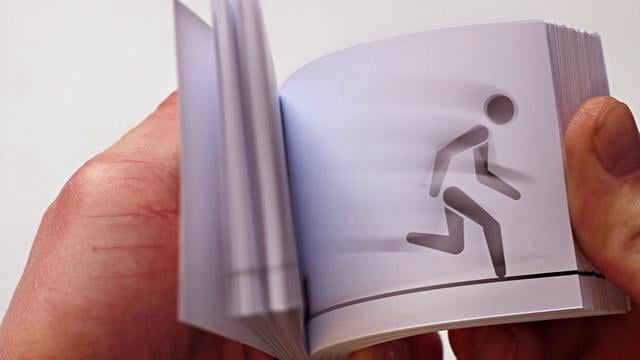
\includegraphics[width = 0.6\textwidth, keepaspectratio]{./img/flipBook.jpg}
%        \caption{A técnica de animação dá vida aos modelos ao posicioná-los em
%          poses ligeiramente diferentes, criando a ilusão do movimento }
%
%       %http://ewanmcgeachie.blogspot.com.br/2015/11/flipbook.html
%      \end{figure}
%
%
%\end{frame}

\begin{frame}[fragile]
  \frametitle{Introdução}

  \begin{itemize}
  	\item Mercado Global de Animação
  		\begin{itemize}
  			\item Rápido crescimento.
  			\item Pode ser dividido em várias categorias:
  			 \begin{itemize}
  				\item Desenvolvimento Web.
  				\item Educação.
  				\item \textbf{Filmes} e \textbf{Efeitos Visuais}. 
   				\end{itemize}
  				\item Técnicas atuais apresentam \textbf{alto custo}.
   		\end{itemize}
  

   \end{itemize}


\end{frame}


\begin{frame}
  Animações computacionais são utilizadas em filmes completamente digitalmente
  animados.
      \begin{figure}
        \centering
        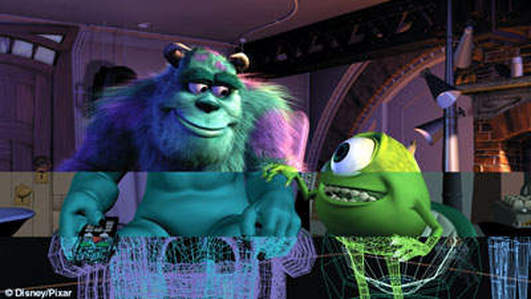
\includegraphics[width = 0.8\textwidth, keepaspectratio]{./img/sully.jpg}
        \caption{Um único quadro com o personagem Sully custou em média de 11 a 12 horas de trabalho criativo (retirado de \cite{sullypixar}).}
      \end{figure}
\end{frame}

%\begin{frame}
%  Ou também para compor filmes onde atores interagem com modelos computacionais.
%      \begin{figure}
%        \centering
%        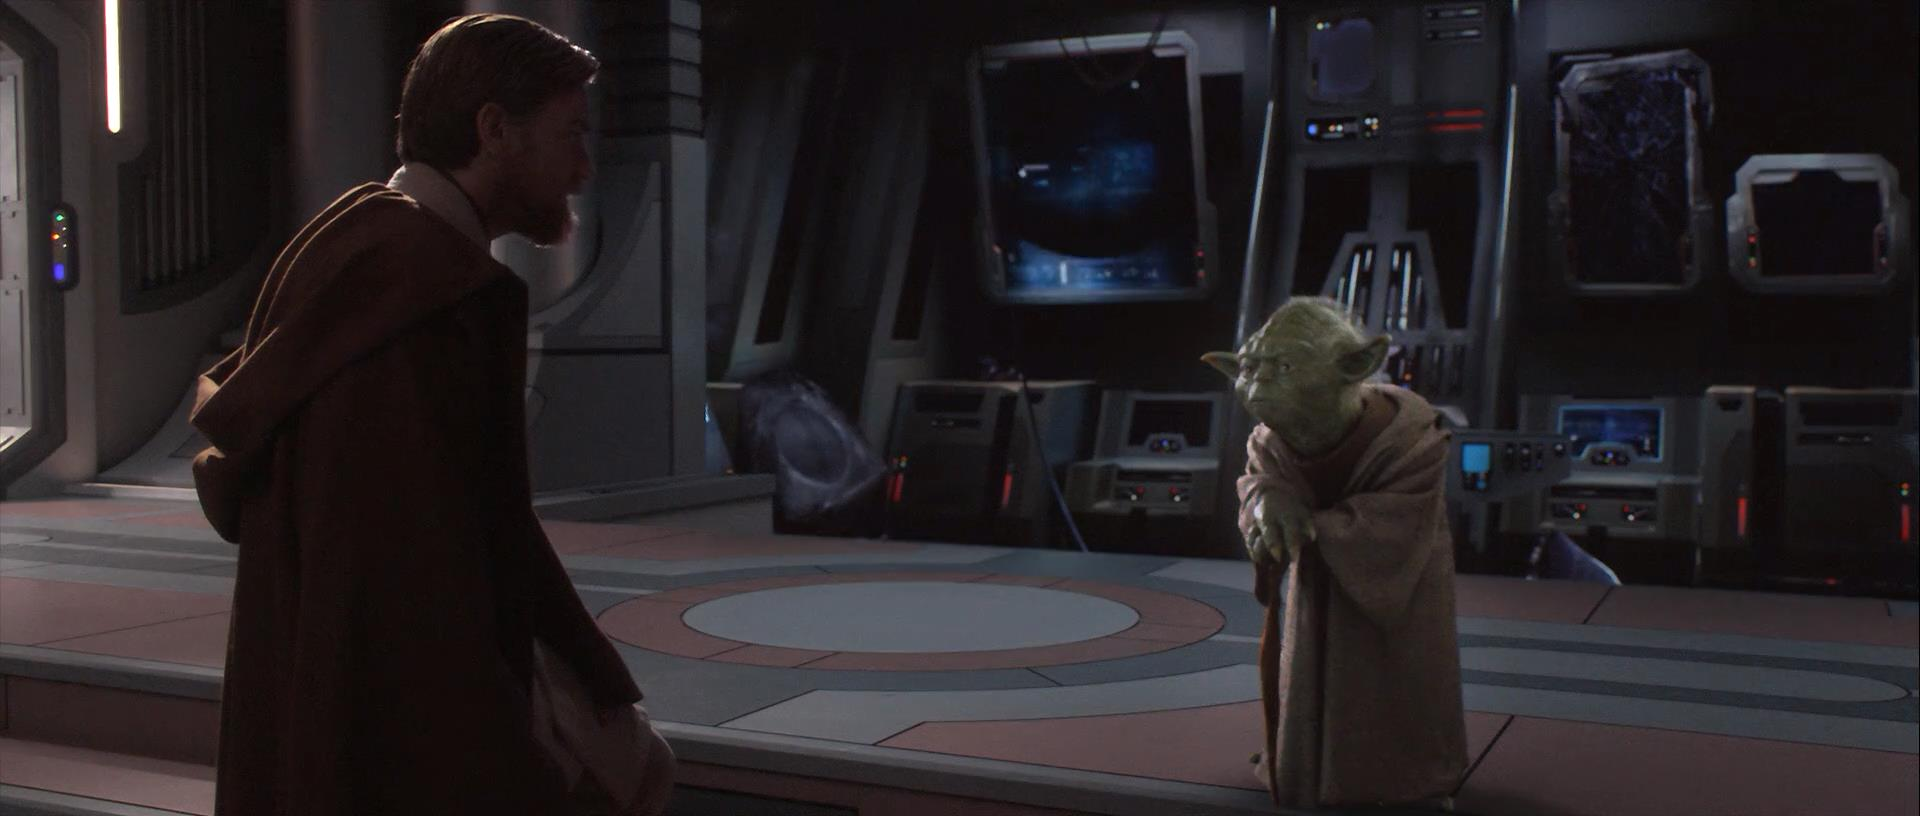
\includegraphics[width = 0.8\textwidth, keepaspectratio]{./img/actorAndAnimation.jpg}
%        \caption{O ator interage com personagem completamente digital.}
%%http://vignette3.wikia.nocookie.net/disney/images/2/28/Yoda_instructs_Obi-Wan_to_kill_Anakin.jpg/revision/latest?cb=20141229172307
%      \end{figure}
%\end{frame}

\begin{frame}
  É possível também transferir movimentos de atores para modelos.
  \begin{figure}[ht]
        \begin{minipage}[b]{0.45\linewidth}
            \centering
            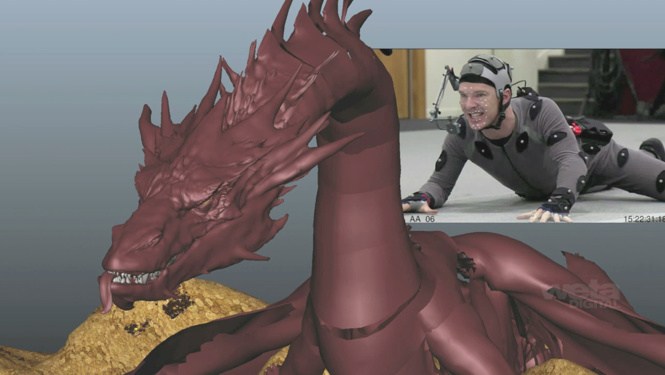
\includegraphics[width = 1.0\textwidth, keepaspectratio]{./img/smaug_left.jpg}
        \end{minipage}
        \begin{minipage}[b]{0.45\linewidth}
          \centering
              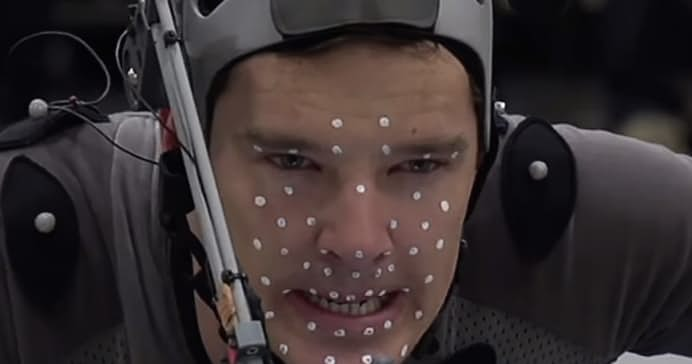
\includegraphics[width = 1.0\textwidth, keepaspectratio]{./img/smaug_right.jpg}
        \end{minipage}

        \caption{Movimentos e expressões são transferidos do ator para o modelo.
       Artistas gráficos dão o retoque final na animação para garantir que o
     resultado seja o mais convincente possível (retirado de \cite{sherlocksmaug}). }
      \end{figure}
\end{frame}


\begin{frame}
  \begin{itemize}
      \item Motivação:
      \begin{itemize}
        \item O \textbf{alto custo} dos produtos existentes é dado, principalmente, por alguns fatores: 
          \begin{itemize}
            \item inúmeras horas de trabalho artístico
            \item equipamentos especiais de captura
            \item ambientes controlados
          \end{itemize}
        \item Esse custo pode se tornar proibitivo para aplicações
          independentes que não dispõe do mesmo orçamento que blockbusters.
      \end{itemize}   
      \item Será que é possível desenvolver um sistema de baixo custo que
        realize transferência de movimento para um avatar computacional?
  \end{itemize} 

\end{frame}


\section{Metodologia}

\subsection{Inspiração}
\begin{frame}
	\frametitle{Vídeo sobre Blend Shapes no Maia}
      \begin{figure}
        \centering
        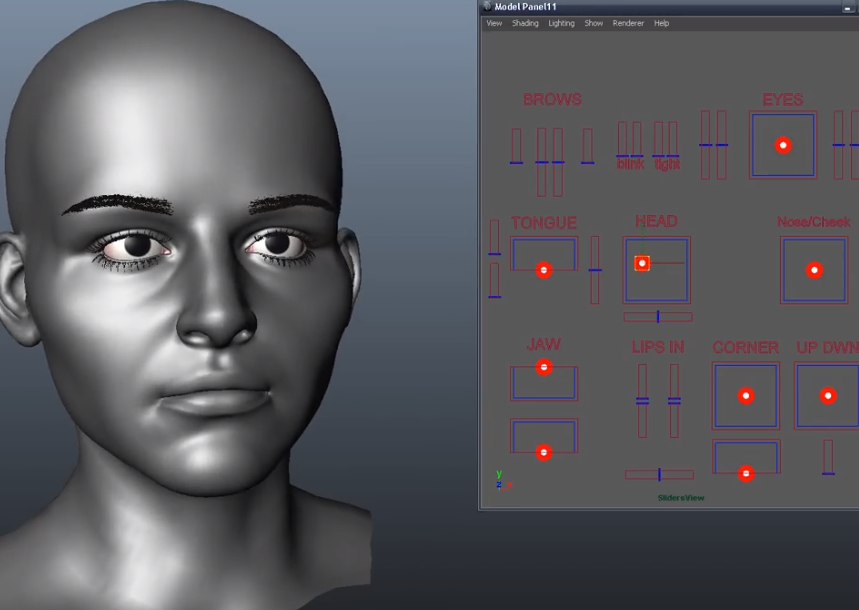
\includegraphics[width = 0.8\textwidth, keepaspectratio]{./img/maiaDemo.png}
      \end{figure}   
\end{frame}

\begin{frame}
 	\frametitle{Metodologia Simplificada}
       \begin{figure}
         \centering
         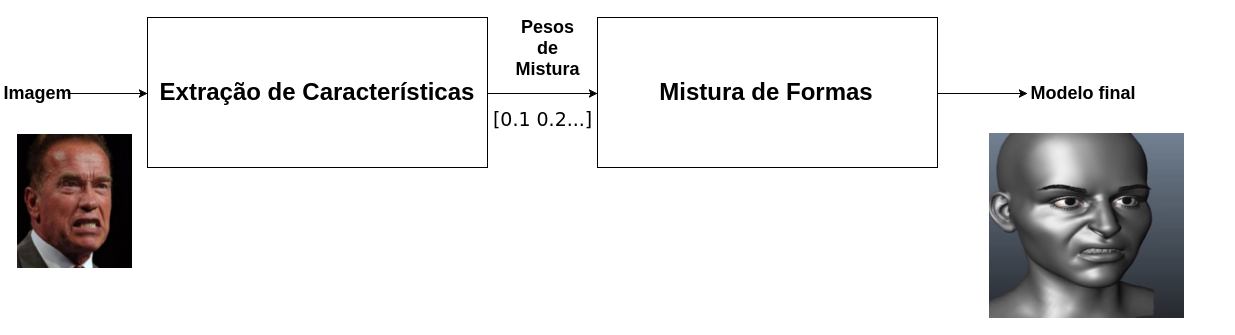
\includegraphics[width = 1.1\textwidth]{./img/EZ3d-simplified.png}
       \end{figure}   
\end{frame}


\begin{frame}
	\frametitle{Metodologia}
      \begin{figure}
        \centering
        \includegraphics[width = 0.9\textwidth, keepaspectratio]{./img/metodologia-slide.png}
      \end{figure}   
\end{frame}

\section{Rastreamento de Pontos Faciais}

\begin{frame}
\frametitle{Rastreamento de Pontos do Rosto}
        \begin{figure}
            \centering
            \includegraphics[width = 0.9\textwidth, keepaspectratio]{./img/metodologia-marcado-pdm.png}
      \end{figure}
\end{frame}

\begin{frame}
\frametitle{Rastreamento de Pontos do Rosto}
        \begin{figure}
            \centering
            \includegraphics[width = 0.8\textwidth, keepaspectratio]{./img/metodologia-destacado-pdm.png}
      \end{figure}
\end{frame}

\begin{frame}
\frametitle{Rastreamento de Pontos do Rosto}
        \begin{figure}
            \centering
            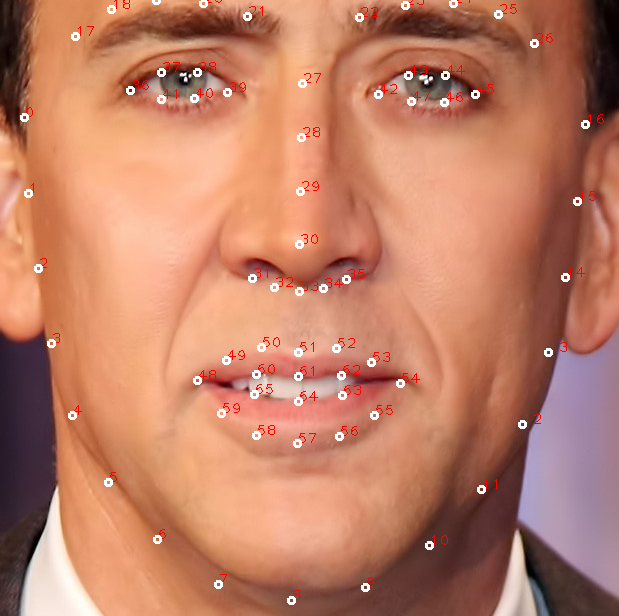
\includegraphics[width = 0.4\textwidth, keepaspectratio]{./img/nick-marked.png}
           \caption{CSIRO Face analysis SDK}
      \end{figure}
\end{frame}


\begin{frame}
\frametitle{Modelo de Distribuição de Pontos - PDM}

\begin{definition}
  O PDM modela linearmente variações de forma não-rígidas e as compõe com uma transformação rígida global, colocando o i-ésimo ponto de interesse
$\bm{v_i}$ em:

\begin{equation}
 \bm{v_i} = s \bm{R} ( \bm{v}_{i,0} + \bm{\Phi}_i \bm{q}) + \bm{t}
\label{eq:PDM-equation}
\end{equation}
\end{definition}
\end{frame}

% http://www.menpo.org/menpofit/pdm.html
\begin{frame}
\frametitle{Rastreamento de Pontos do Rosto}
      \begin{figure}
          \centering
          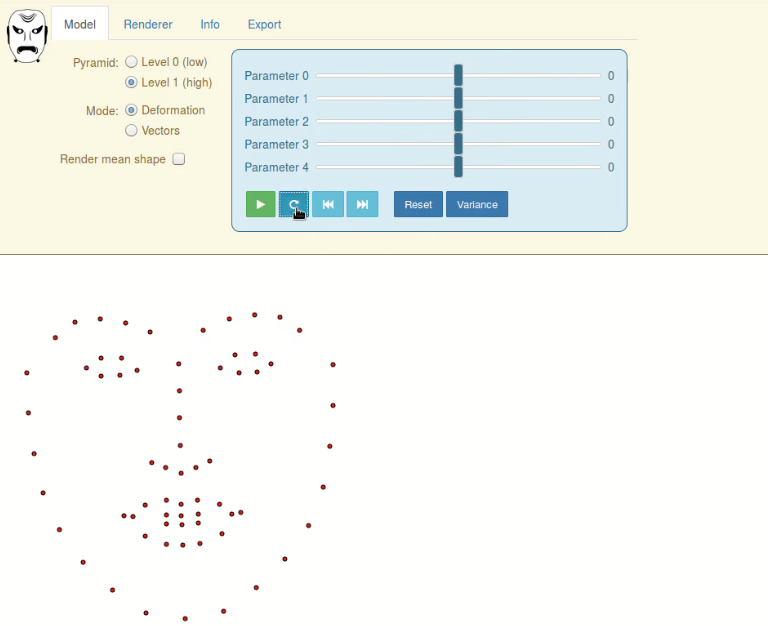
\includegraphics[width = 0.6\textwidth, keepaspectratio]{./img/pca_exaplained.png}
          \caption{Visualização das componentes de deformação aprendidas pela análise PCA.}
      \end{figure}
\end{frame}

\begin{frame}
\frametitle{Razão de Distância}
        \begin{figure}
            \centering
            \includegraphics[width = 0.9\textwidth, keepaspectratio]{./img/metodologia-marcado-razaodist.png}
      \end{figure}
\end{frame}

\begin{frame}
\frametitle{Razão de Distância}
        \begin{figure}
            \centering
            \includegraphics[width = 0.8\textwidth, keepaspectratio]{./img/metodologia-destacado-razaodist.png}
      \end{figure}
\end{frame}

\begin{frame}
\frametitle{Razão de Distância}

\begin{block}{Razão de Distância}
  O objetivo desta etapa é extrair informação dos 66 pontos rastreados de forma
  a construir os coeficientes de mistura necessários para a Mistura de Poses
\end{block}
\end{frame}

\begin{frame}
\frametitle{Razão de Distância}
  \begin{itemize}
      \item Em uma etapa de calibração, mede-se o máximo e o mínimo da
        distância de interesse a atribui-se a essas os valores de 1 e 0.
      \item Uma regra de proporção é utilizada para calcular poses
        intermediárias
  \end{itemize} 
\end{frame}

\begin{frame}
\frametitle{Razão de Distância}
  \begin{itemize}
      \item distância entre os 2 pontos de interesse deve ser normalizada 
        para o intervalo $[0, 1]$.

      \item Em uma etapa de calibração, mede-se a distância entre os pontos em
        condições extremas.
  \end{itemize} 
\end{frame}

\begin{frame}
\frametitle{Razão de Distância}
  \begin{itemize}
      \item Em cada iteração do programa utiliza-se uma regra de proporção para
        calcular o coeficiente de mistura:

\begin{equation}
	w_i^j = \frac{|d_i^j - d_i^{\text{min}}|}{|d_i^{\text{max}} - d^{\text{min}}|}
   \label{eq:pesos1}
\end{equation}

  \end{itemize} 
\end{frame}

\begin{frame}
\frametitle{Mistura de Poses}
        \begin{figure}
            \centering
            \includegraphics[width = 0.9\textwidth, keepaspectratio]{./img/metodologia-marcado-MP.png}
      \end{figure}
\end{frame}

\begin{frame}
\frametitle{Mistura de Poses}
        \begin{figure}
            \centering
            \includegraphics[width = 0.8\textwidth, keepaspectratio]{./img/metodologia-destacado-MP.png}
      \end{figure}
\end{frame}



\begin{frame}
  \begin{itemize}
  \item Mistura de Poses:
  \begin{figure}
\centering
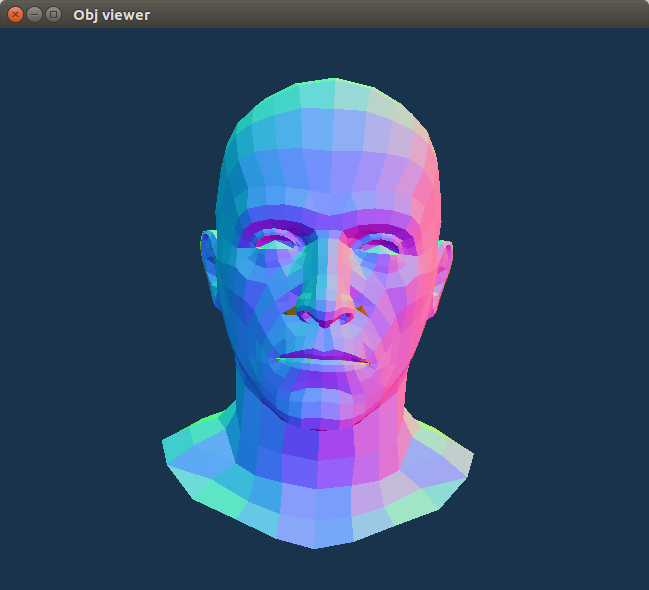
\includegraphics[width = 0.6\textwidth, keepaspectratio]{./img/rosto-neutro.png}
        \caption{Pose Neutra}
     \end{figure}         
  \end{itemize} 
\end{frame}

\begin{frame}
  \begin{itemize}
  \item Mistura de Poses:
  \begin{figure}
\centering
      \begin{tabular}{ccc}
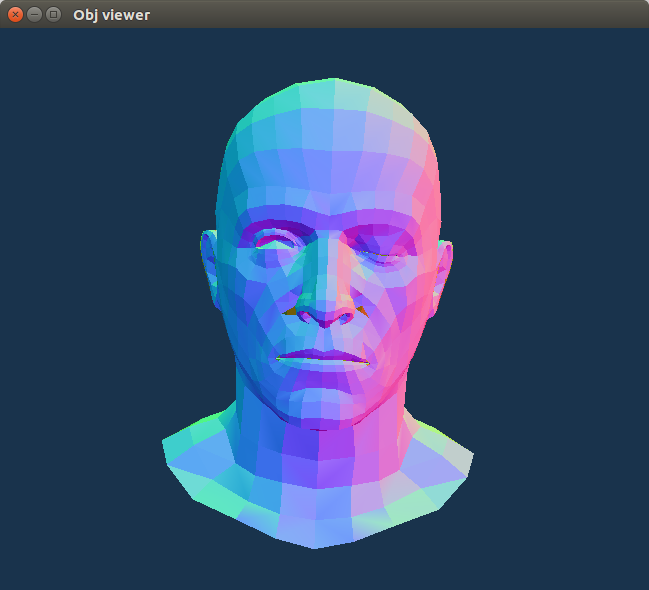
\includegraphics[width=0.3\linewidth]{./img/left-closed-eye.png} &
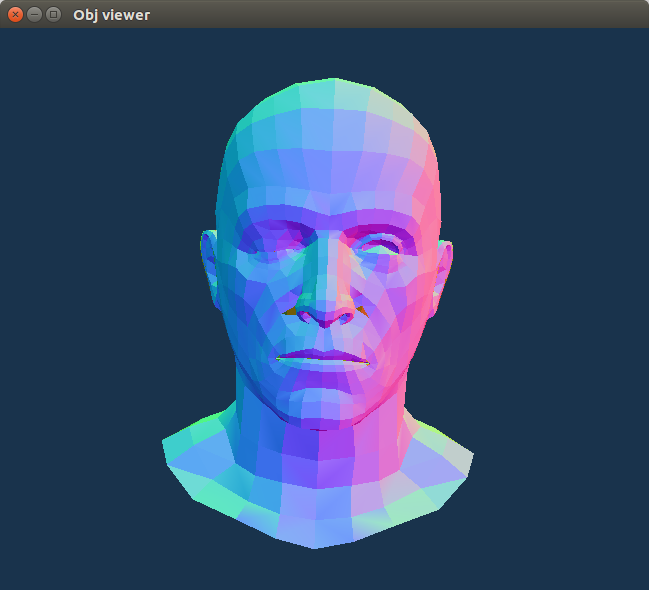
\includegraphics[width=0.3\linewidth]{./img/right-closed-eye.png} &
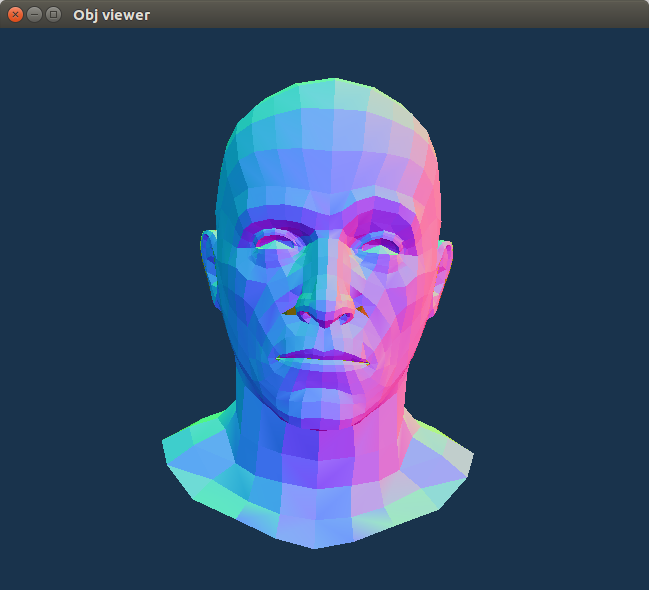
\includegraphics[width=0.3\linewidth]{./img/left-eyebrow.png} \\
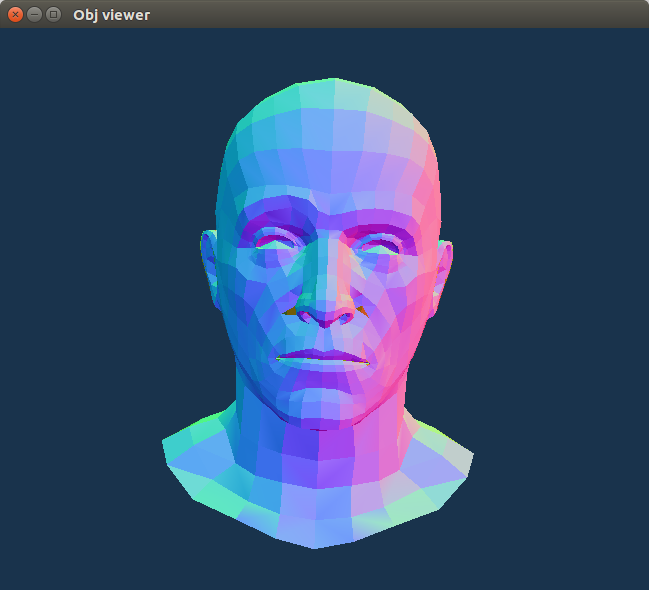
\includegraphics[width=0.3\linewidth]{./img/right-eyebrow.png} &
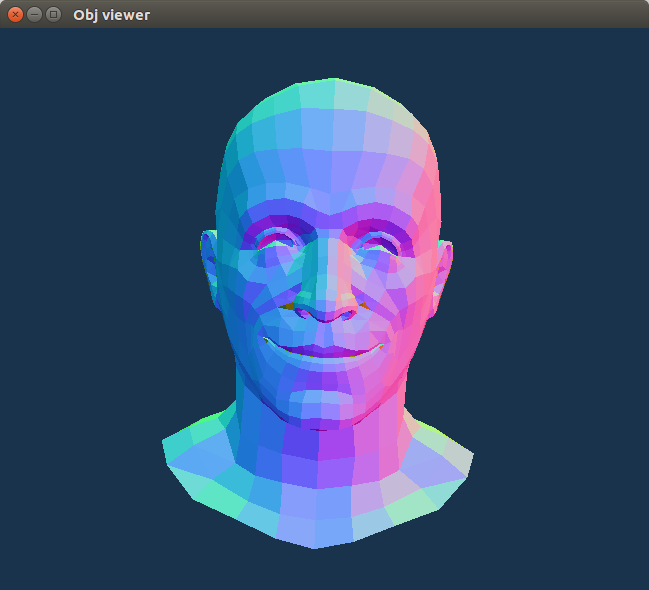
\includegraphics[width=0.3\linewidth]{./img/rosto-feliz.png} &
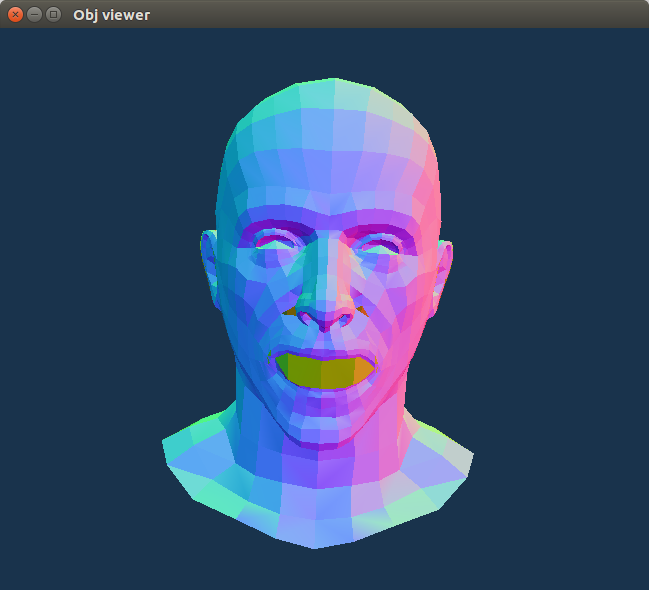
\includegraphics[width=0.3\linewidth]{./img/open-mouth.png} \\
	\end{tabular}
	\caption{Poses pré definidas utilizadas neste trabalho}
     \end{figure}         
  \end{itemize} 
\end{frame}

\begin{frame}
  \begin{itemize}
  \item Mistura de Poses:
  \begin{figure}
\centering
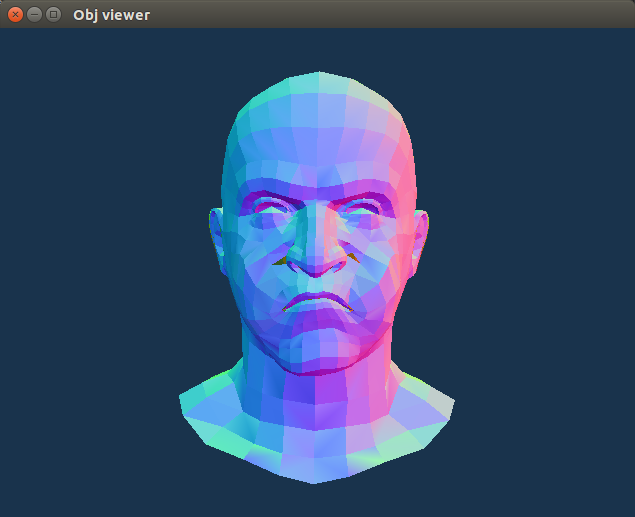
\includegraphics[width = 0.6\textwidth, keepaspectratio]{./img/poseCombinada.png}
        \caption{Exemplo de combinação possível. }
     \end{figure}         
  \end{itemize} 
\end{frame}

\begin{frame}
\frametitle{Mistura de Poses}

	\begin{figure}
        \centering
        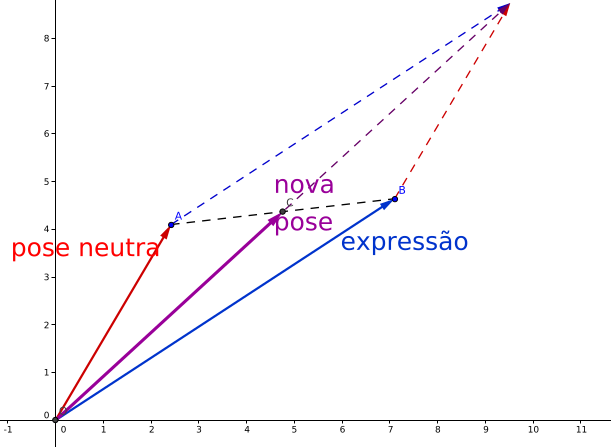
\includegraphics[width = 0.7\textwidth, keepaspectratio]{./img/vectors00.png}
        \caption{A combinação dos vetores é feita de forma que o resultado seja
          um ponto sobre linha que conecta o primeiro ao segundo vetor.}
      \end{figure}
\end{frame}

\begin{frame}
\frametitle{Mistura de Poses}

        O resultado anterior não é coincidência: 
          $$ (1 - w)\vec{A} + w \vec{B} = \vec{A} + w (\vec{B} -
          \vec{A})$$

	\begin{figure}
        \centering
        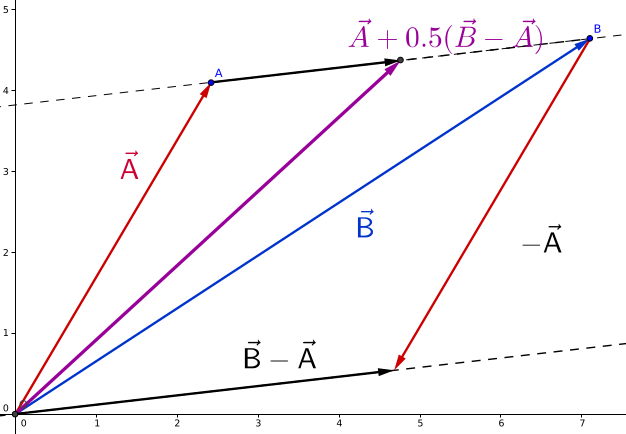
\includegraphics[width = 0.6\textwidth, keepaspectratio]{./img/vectors01.png}
        \caption{Ilustração da propriedade para $w = 0.5$}
      \end{figure}
\end{frame}
 
\begin{frame}
\frametitle{Mistura de Poses}
  \begin{itemize}
  	\item Mistura de Formas( Blend Shapes ou Morph Target ):
 	 	\begin{itemize}
        \item Técnica de animação comumente empregadas para modelar objetos como a \textbf{face humana}.
        \item gera poses intermediárias como uma \textbf{combinação linear} de poses pré-definidas. 
  \end{itemize} 

  \end{itemize} 
\end{frame}

\begin{frame}
\frametitle{Mistura de Poses}
 	 	\begin{itemize}
  	    \item A mistura vetorial acontece ponto a ponto.
          
        \item Sendo $\vec{M}_j^i$ o j-ésimo ponto da i-ésima pose, o j-ésimo
          ponto da mistura $\vec{J}_j$ pode ser obtido por:

      
          \begin{equation}
            \vec{J}_j = \sum_{i=1}^L  w_i \vec{M}_j^i
          \end{equation}

          \item O peso para a pose neutra é escolhido de forma a normalizar a
            soma dos pesos:
            \begin{equation}
              w_1 = 1 - \sum_{i=2}^L w_i
            \end{equation}
          
    \end{itemize} 
\end{frame}

\begin{frame}
\frametitle{Mistura de Poses}
  \begin{itemize}
  	
  	\item Mistura de Formas( Blend Shapes ou Morph Target ):
  	
  	
 	 	\begin{itemize}
          \item Com essa condição, pode-se obter a seguinte forma equivalente:
      
          \begin{equation}
            \vec{J}_j = \vec{M}_1 + \sum_{i = 2}^L w_i \Delta \vec{M}_j^i 
          \end{equation}

    \end{itemize} 

  \end{itemize} 
\end{frame}

\begin{frame}
\frametitle{Estimação de Tridimensionalidade}
        \begin{figure}
            \centering
            \includegraphics[width = 0.9\textwidth, keepaspectratio]{./img/metodologia-marcado-3d.png}
      \end{figure}
\end{frame}

\begin{frame}
\frametitle{Estimação de Tridimensionalidade}      

 \begin{figure}
            \centering
            \includegraphics[width = 0.8\textwidth, keepaspectratio]{./img/metodologia-destacado-3d.png}
      \end{figure}
\end{frame}

\begin{frame}
\frametitle{Estimação de Tridimensionalidade}
  \begin{itemize}
      \item Triangulação:
      
      \begin{figure}
        \centering
        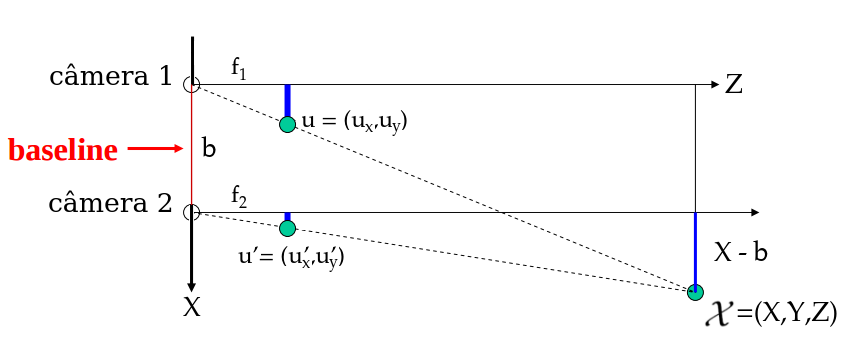
\includegraphics[width = 0.8\textwidth, keepaspectratio]{./img/TG_triangulation_pdf_washington_pt2.png}
      \end{figure}
      
      $X = (u_x/f_1)  Z$ ou $ X = (u'_x/f_2)  Z + b $
      
      $Y = (u_y/f_1) Z$ ou $ Y = (u'_y/f_2) Z$
      
      $Z = f_1  f_2  b / (u_x  f_2 - u'_x  f_1)$
      
  \end{itemize} 
\end{frame}

\begin{frame}
\frametitle{Estimação de Tridimensionalidade}
  \begin{itemize}
      \item Calibração dos Parâmetros Intrínsecos:
      \begin{figure}
        \centering
        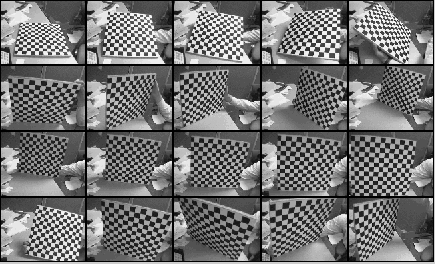
\includegraphics[width = 0.6\textwidth, keepaspectratio]{./img/TG_calib_images.png}
      \end{figure}
  \end{itemize} 
\end{frame}

\begin{frame}
\frametitle{Filtros}
        \begin{figure}
            \centering
            \includegraphics[width = 0.9\textwidth, keepaspectratio]{./img/metodologia-marcado-filtros.png}
      \end{figure}
\end{frame}

\begin{frame}
\frametitle{Filtros}      

 \begin{figure}
            \centering
            \includegraphics[width = 0.6\textwidth, keepaspectratio]{./img/metodologia-destacado-filtros.png}
      \end{figure}
\end{frame}

\begin{frame}
\frametitle{Filtros}
      \begin{figure}
\centering
      \begin{tabular}{cc}
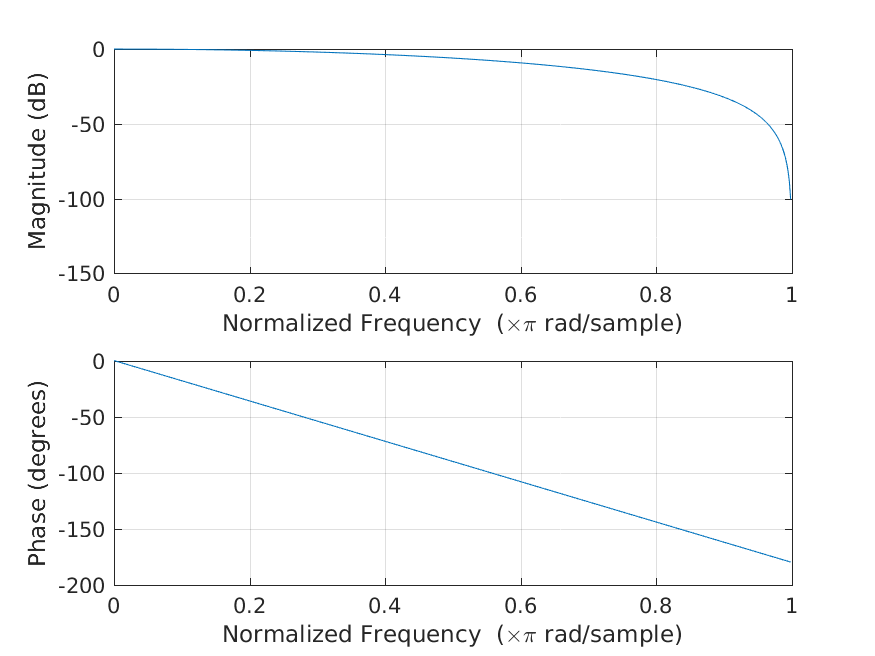
\includegraphics[width=0.35\linewidth]{./img/filter-response-hanningFilter.png} &
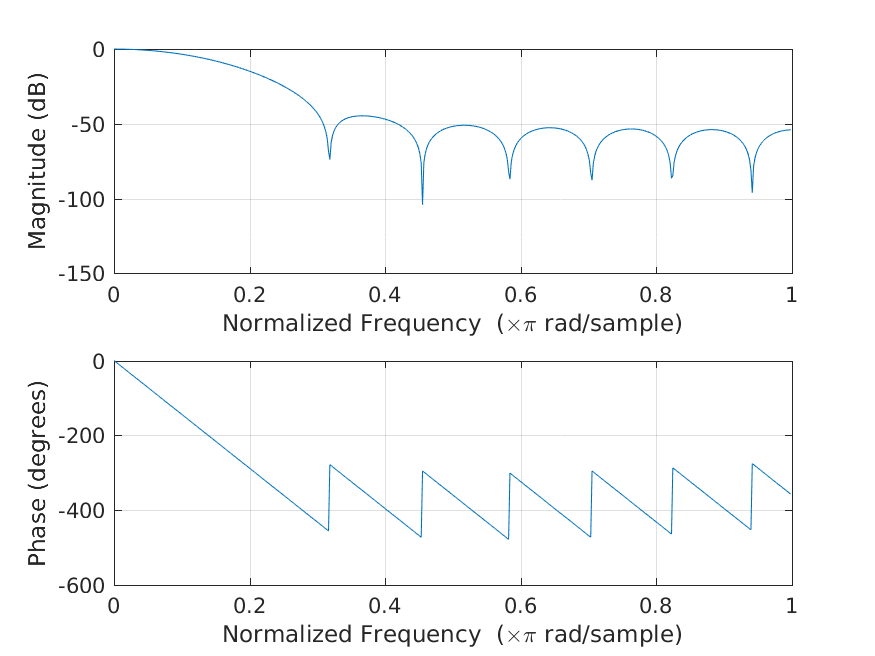
\includegraphics[width=0.35\linewidth]{./img/filter-response-wc_0_1pi.png} \\
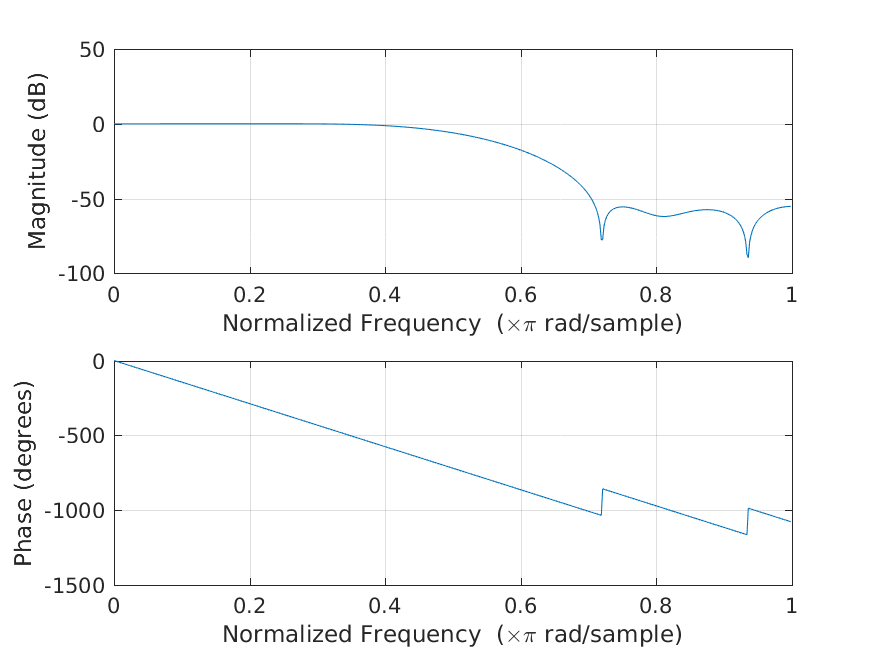
\includegraphics[width=0.35\linewidth]{./img/filter-response-wc_0_5pi.png} &
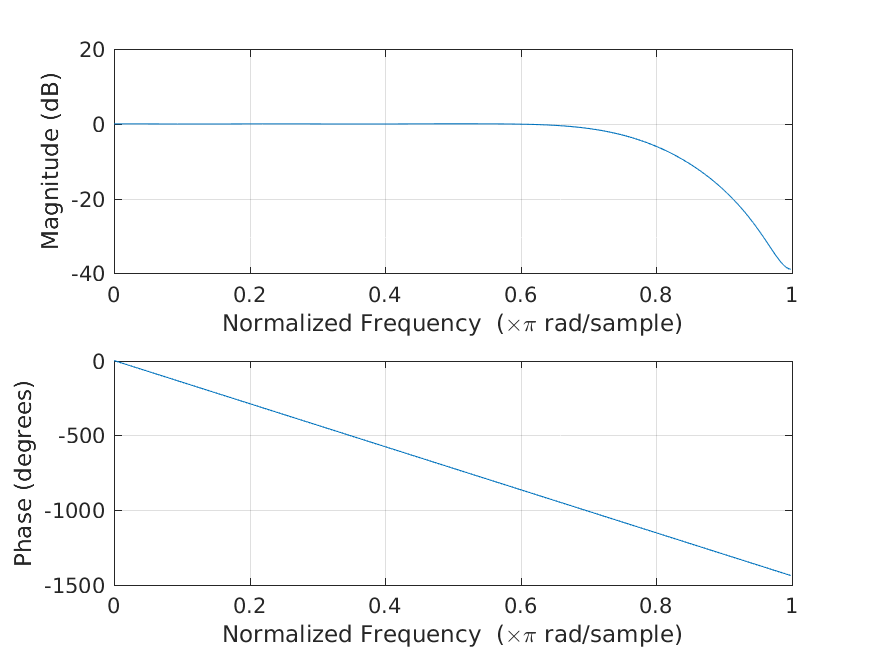
\includegraphics[width=0.35\linewidth]{./img/filter-response-wc_0_8pi.png} \\
	\end{tabular}
	\caption{Respostas aos filtros projetados}
     \end{figure}  
      
\end{frame}

\begin{frame}
\frametitle{Experimento}
	\begin{figure}
        \centering
        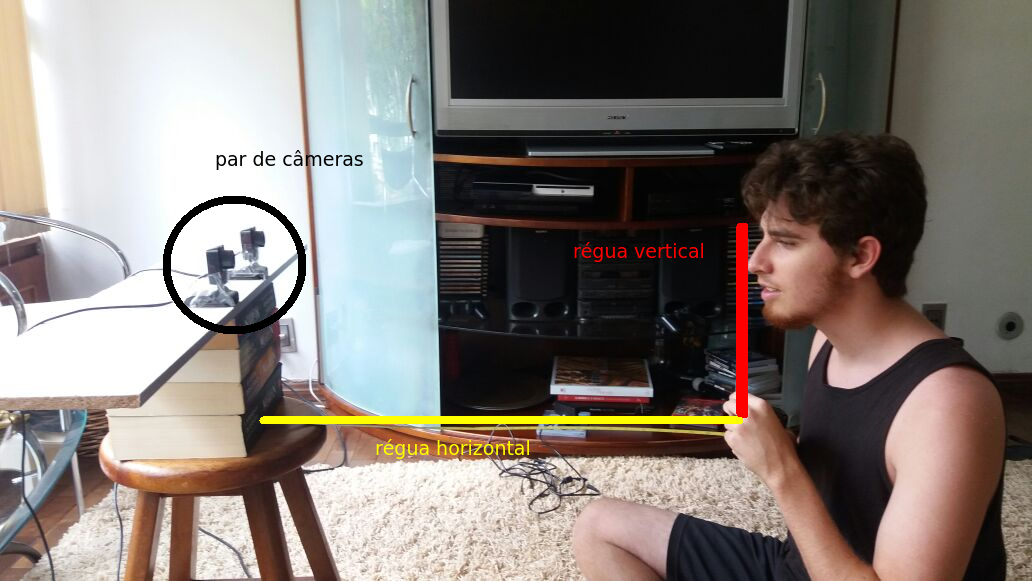
\includegraphics[width = 0.5\textwidth, keepaspectratio]{./img/setup-exp.png}
      \end{figure}
  \begin{enumerate}
  

\item A montagem inicial é executada posicionando o nariz do alvo a 40 centímetros de distância.
\item Capturam-se 30 quadros de cada câmera enquanto o alvo se mantém o mais estático possível.
\item Repete-se o processo com o alvo se afastando 5 centímetros em cada etapa, até que se atinja a distância de 80 cm.
  \end{enumerate} 
\end{frame}

\begin{frame}
\frametitle{Resultados}
  \begin{itemize}
      \item Rastreamento de Pontos do Rosto:
      
       \begin{figure}
        \centering
        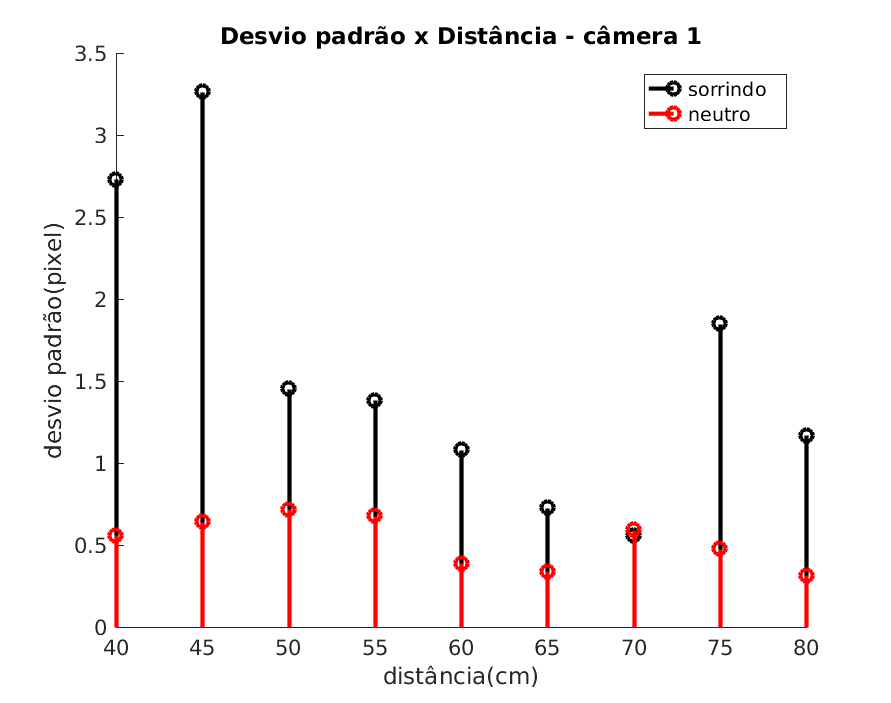
\includegraphics[width = 0.6\textwidth, keepaspectratio]{./img/desvio_cameraEsquerda.jpg}
      \end{figure}
          
  \end{itemize} 
\end{frame}

\begin{frame}
\frametitle{Resultados}
  \begin{itemize}
      \item Rastreamento de Pontos do Rosto:
      
       \begin{figure}
        \centering
        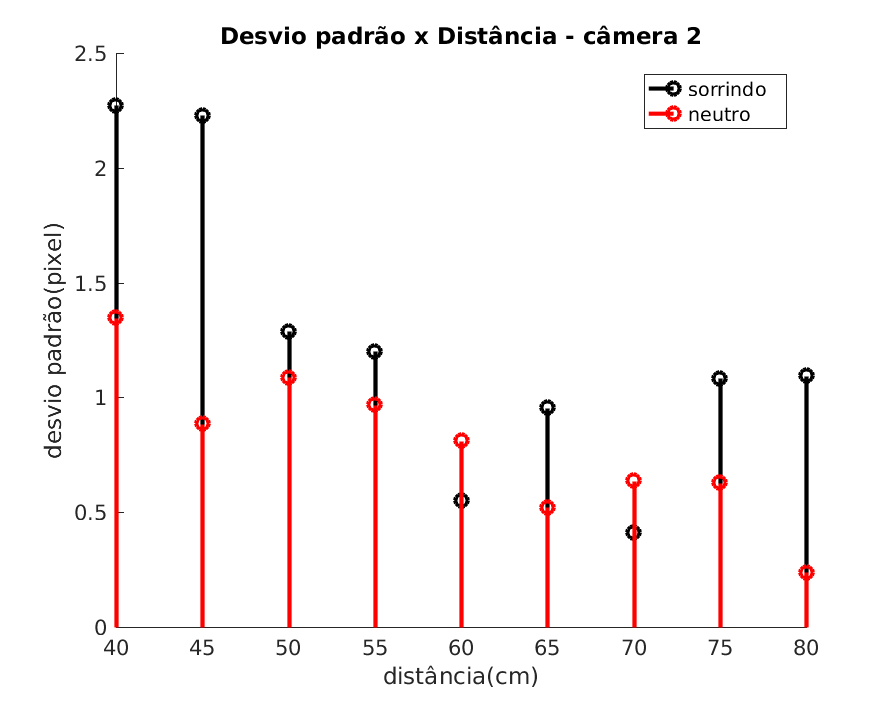
\includegraphics[width = 0.6\textwidth, keepaspectratio]{./img/desvio_cameraDireita.jpg}
      \end{figure}
          
  \end{itemize} 
\end{frame}

\begin{frame}
\frametitle{Estabilização do Rastreamento}
  \begin{itemize}
      \item Estimação da Tridimensionalidade:
      \begin{figure}
        \centering
        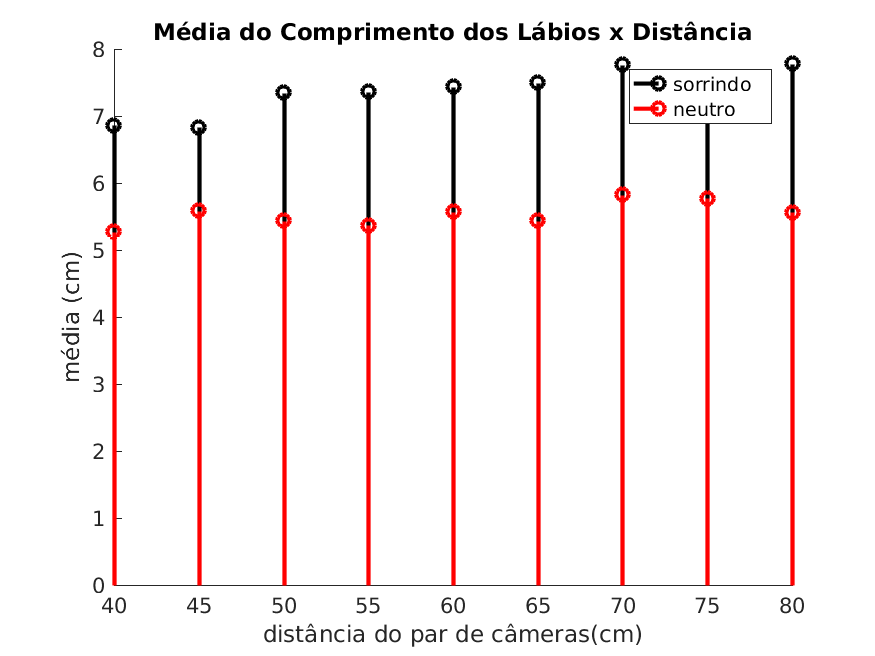
\includegraphics[width = 0.6\textwidth, keepaspectratio]{./img/media_3d.png}
      \end{figure}
               
  \end{itemize} 
\end{frame}

\begin{frame}
  \begin{itemize}
      \item Filtros:
      \begin{figure}
\centering
\begin{tabular}{c}
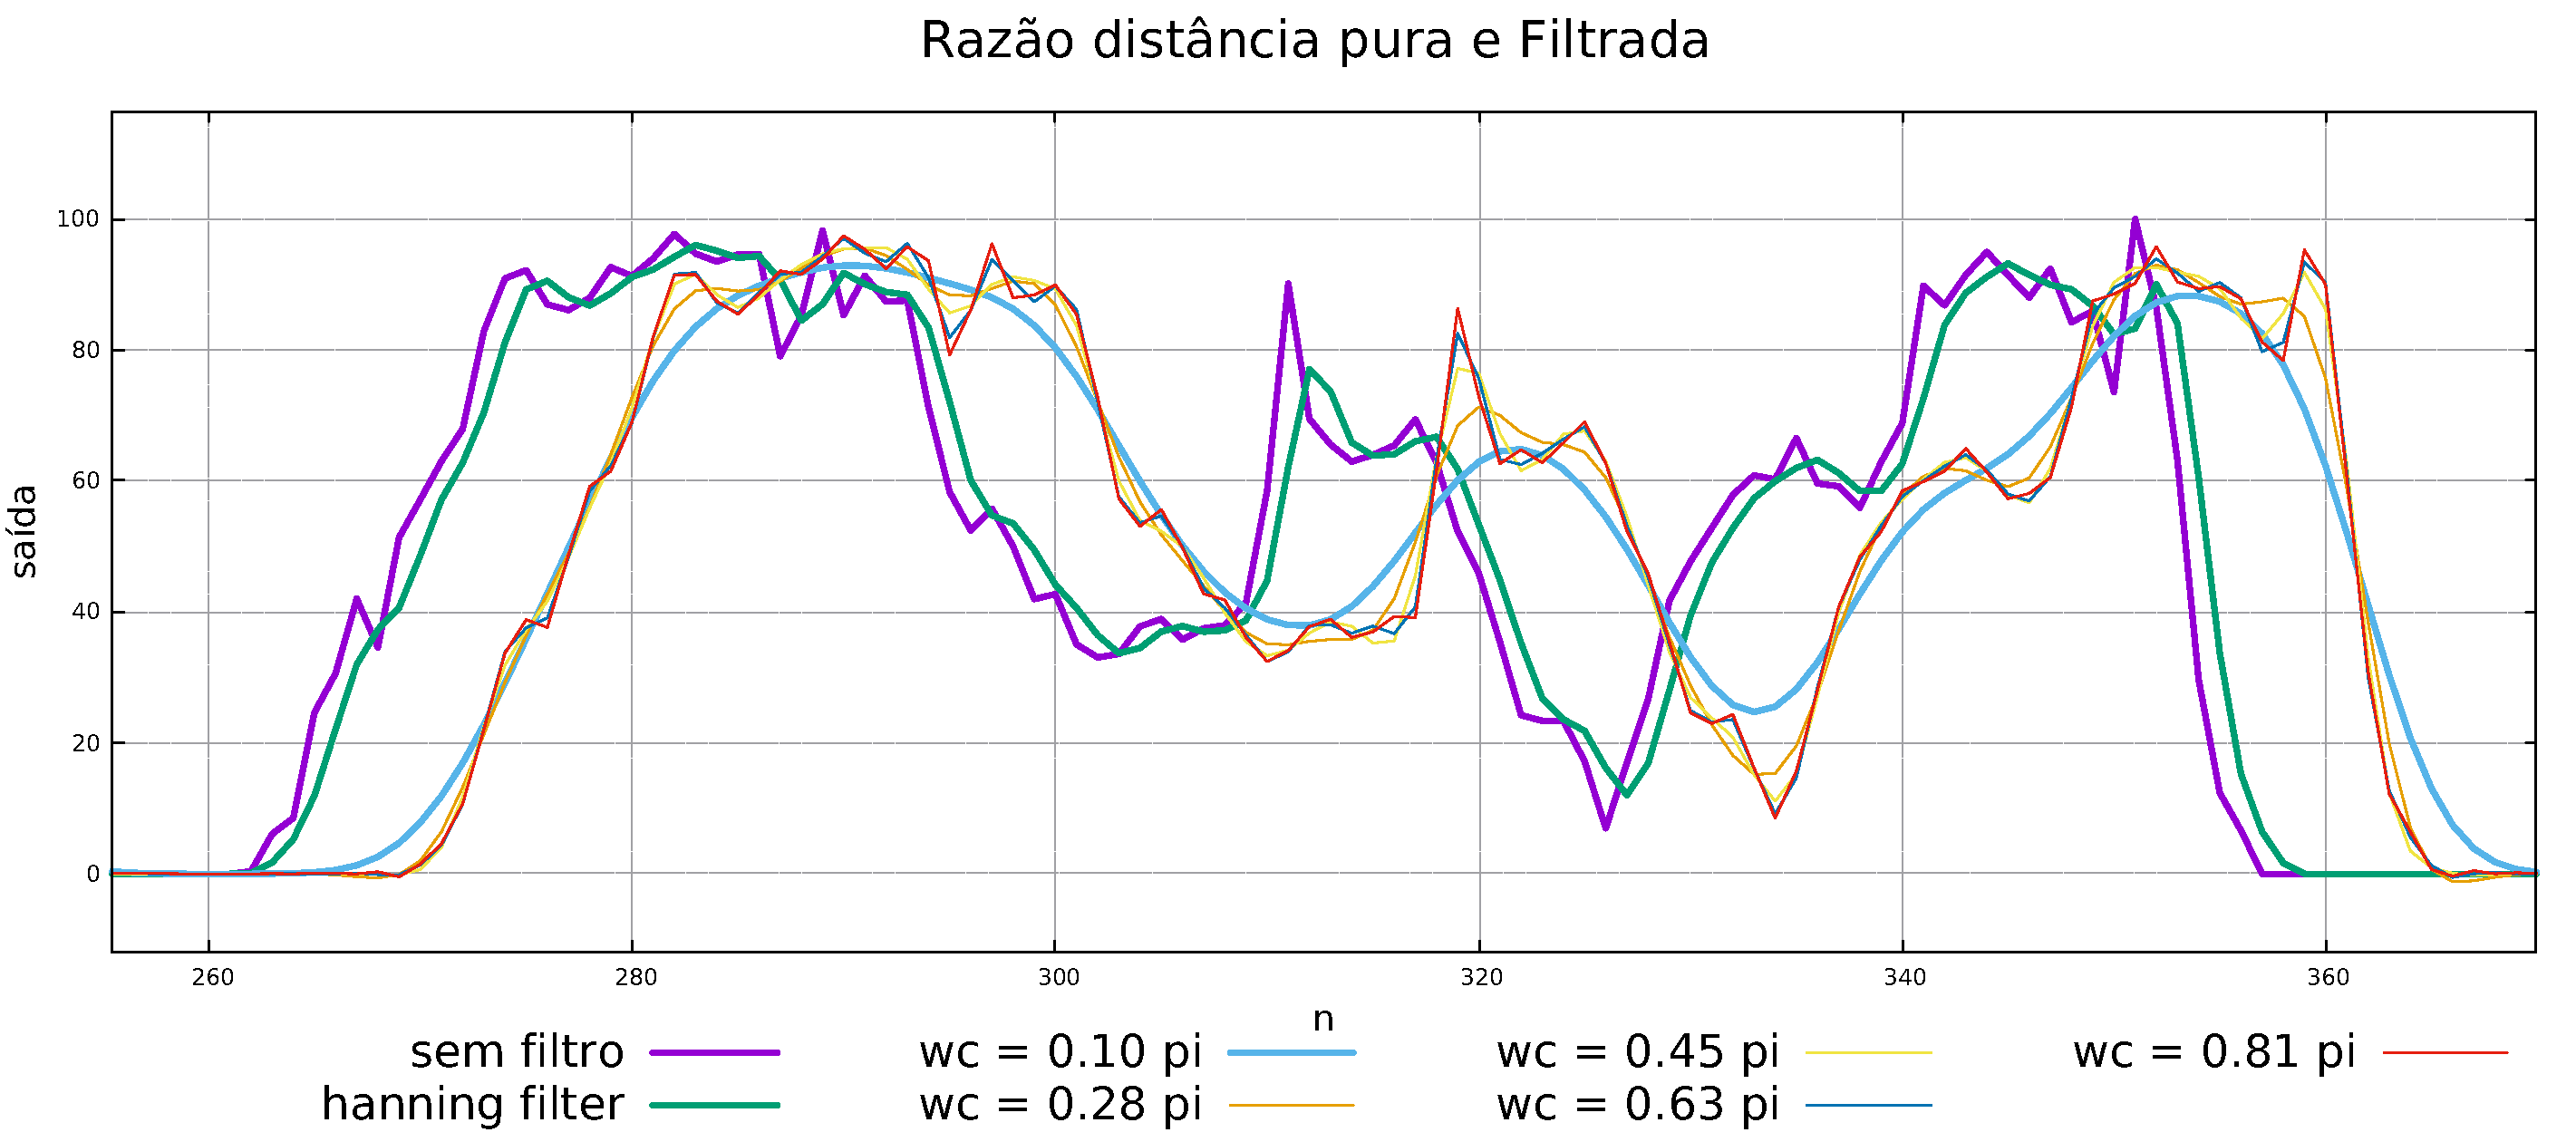
\includegraphics[width=0.6\linewidth]{./img/filter-result-left-eye.pdf} \\
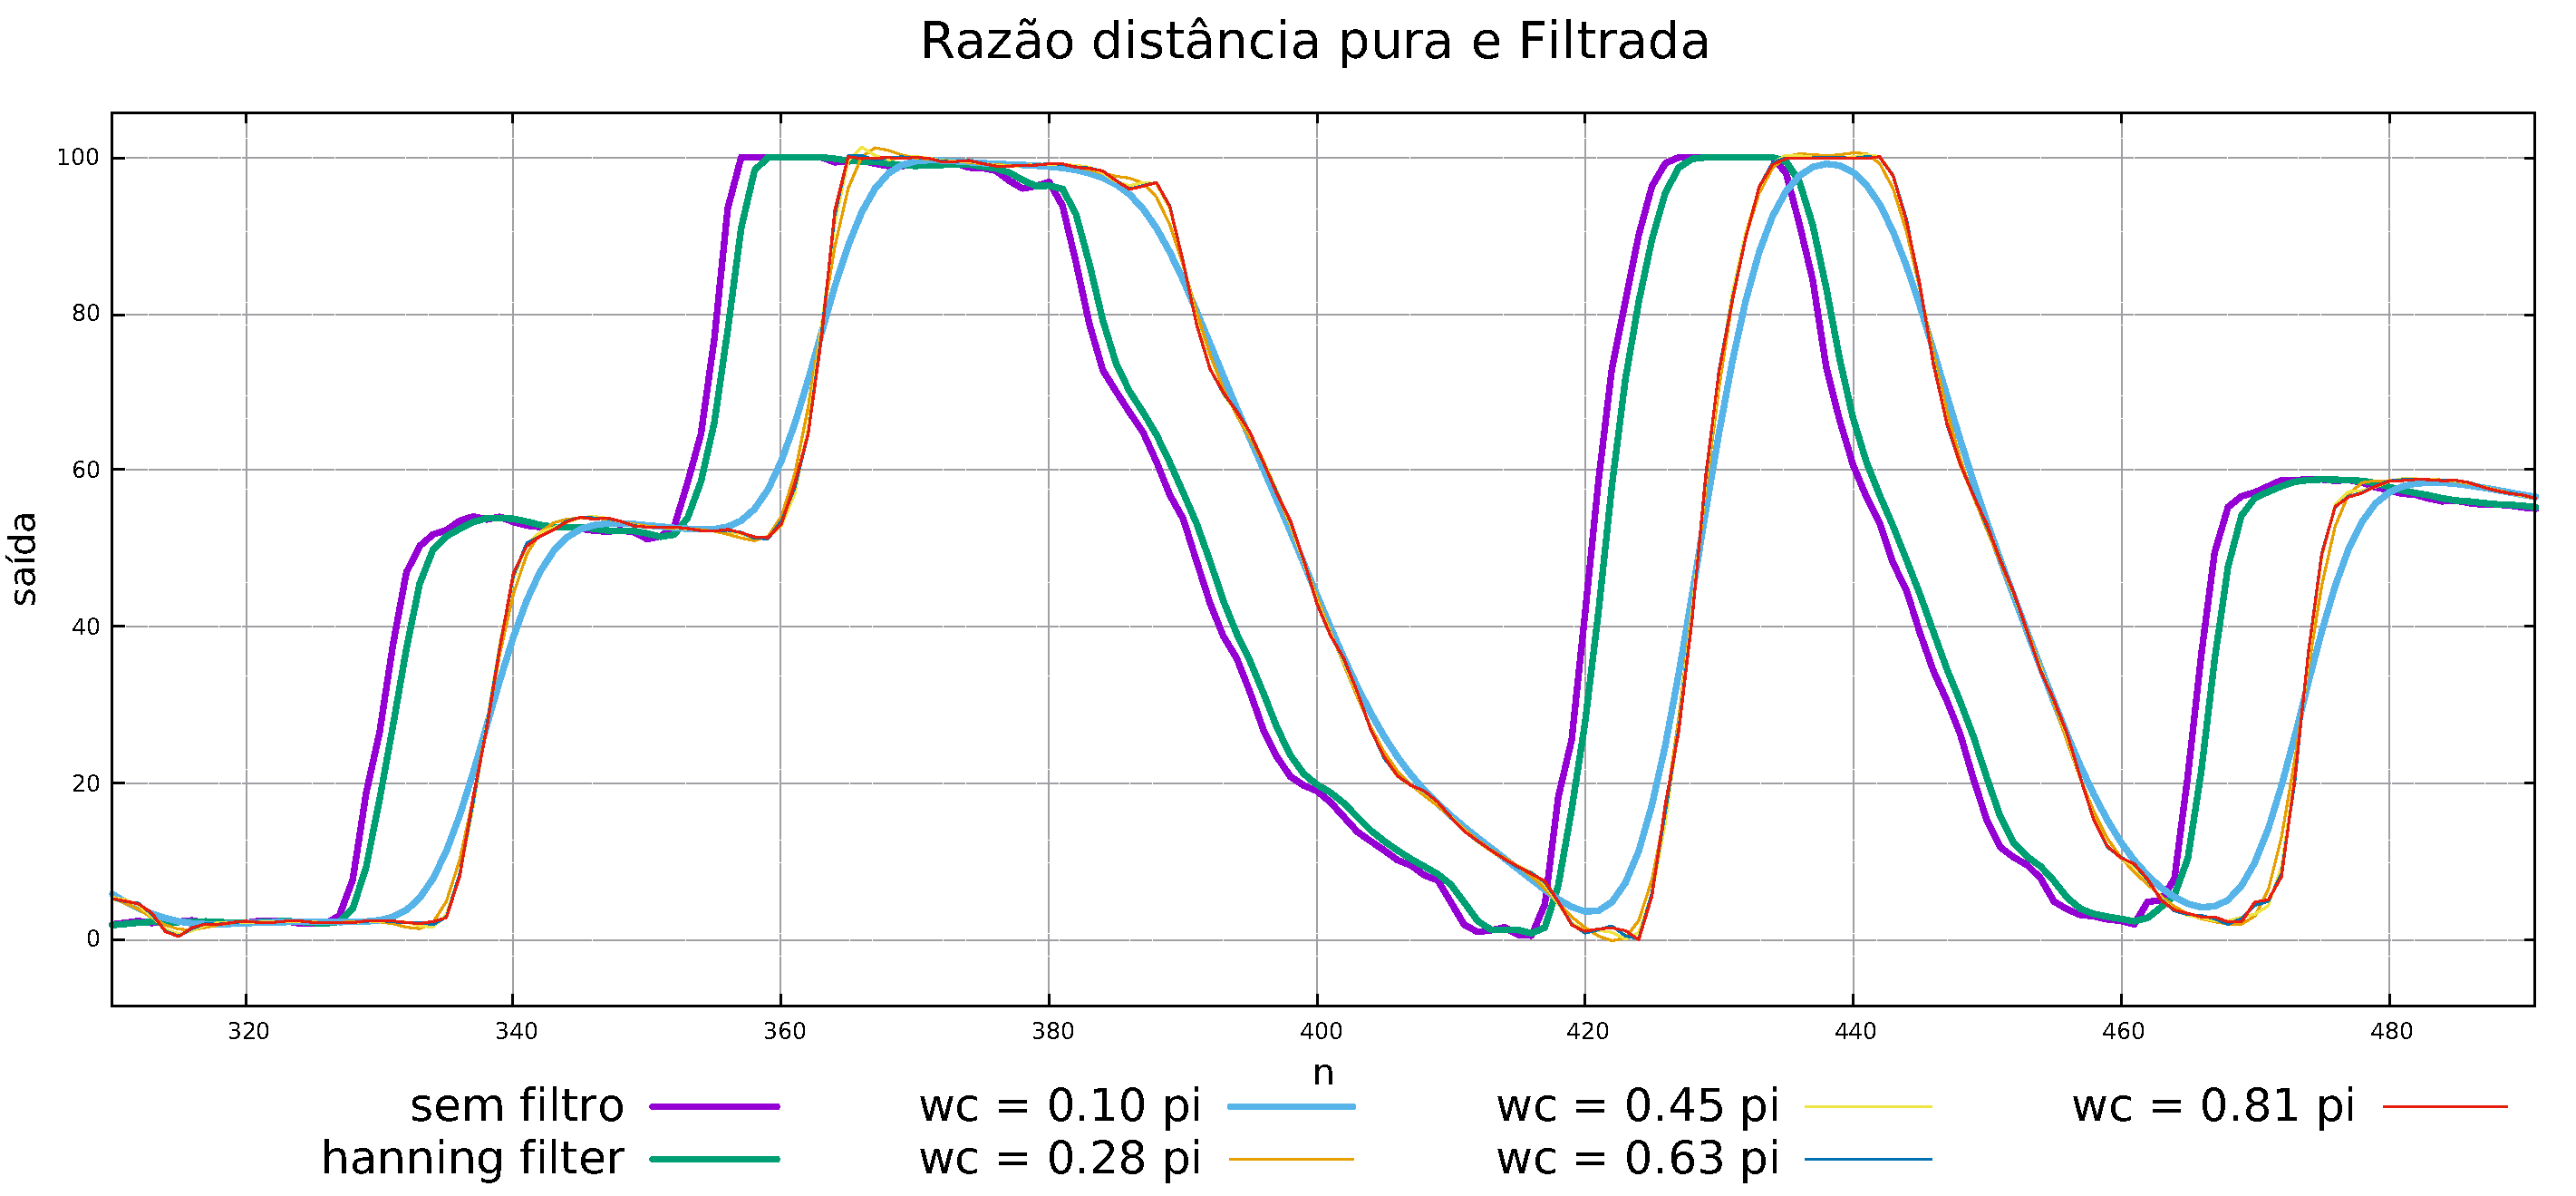
\includegraphics[width=0.6\linewidth]{./img/filter-result-open-mouth.pdf} \\
\end{tabular}
\caption{Resultado da resposta ao sinal dos filtros projetados para o movimento do olho esquerdo e da boca}
\end{figure}
              
  \end{itemize} 
\end{frame}

\begin{frame}
  \begin{itemize}
      \item Filtros:
	\begin{figure}
        \centering
        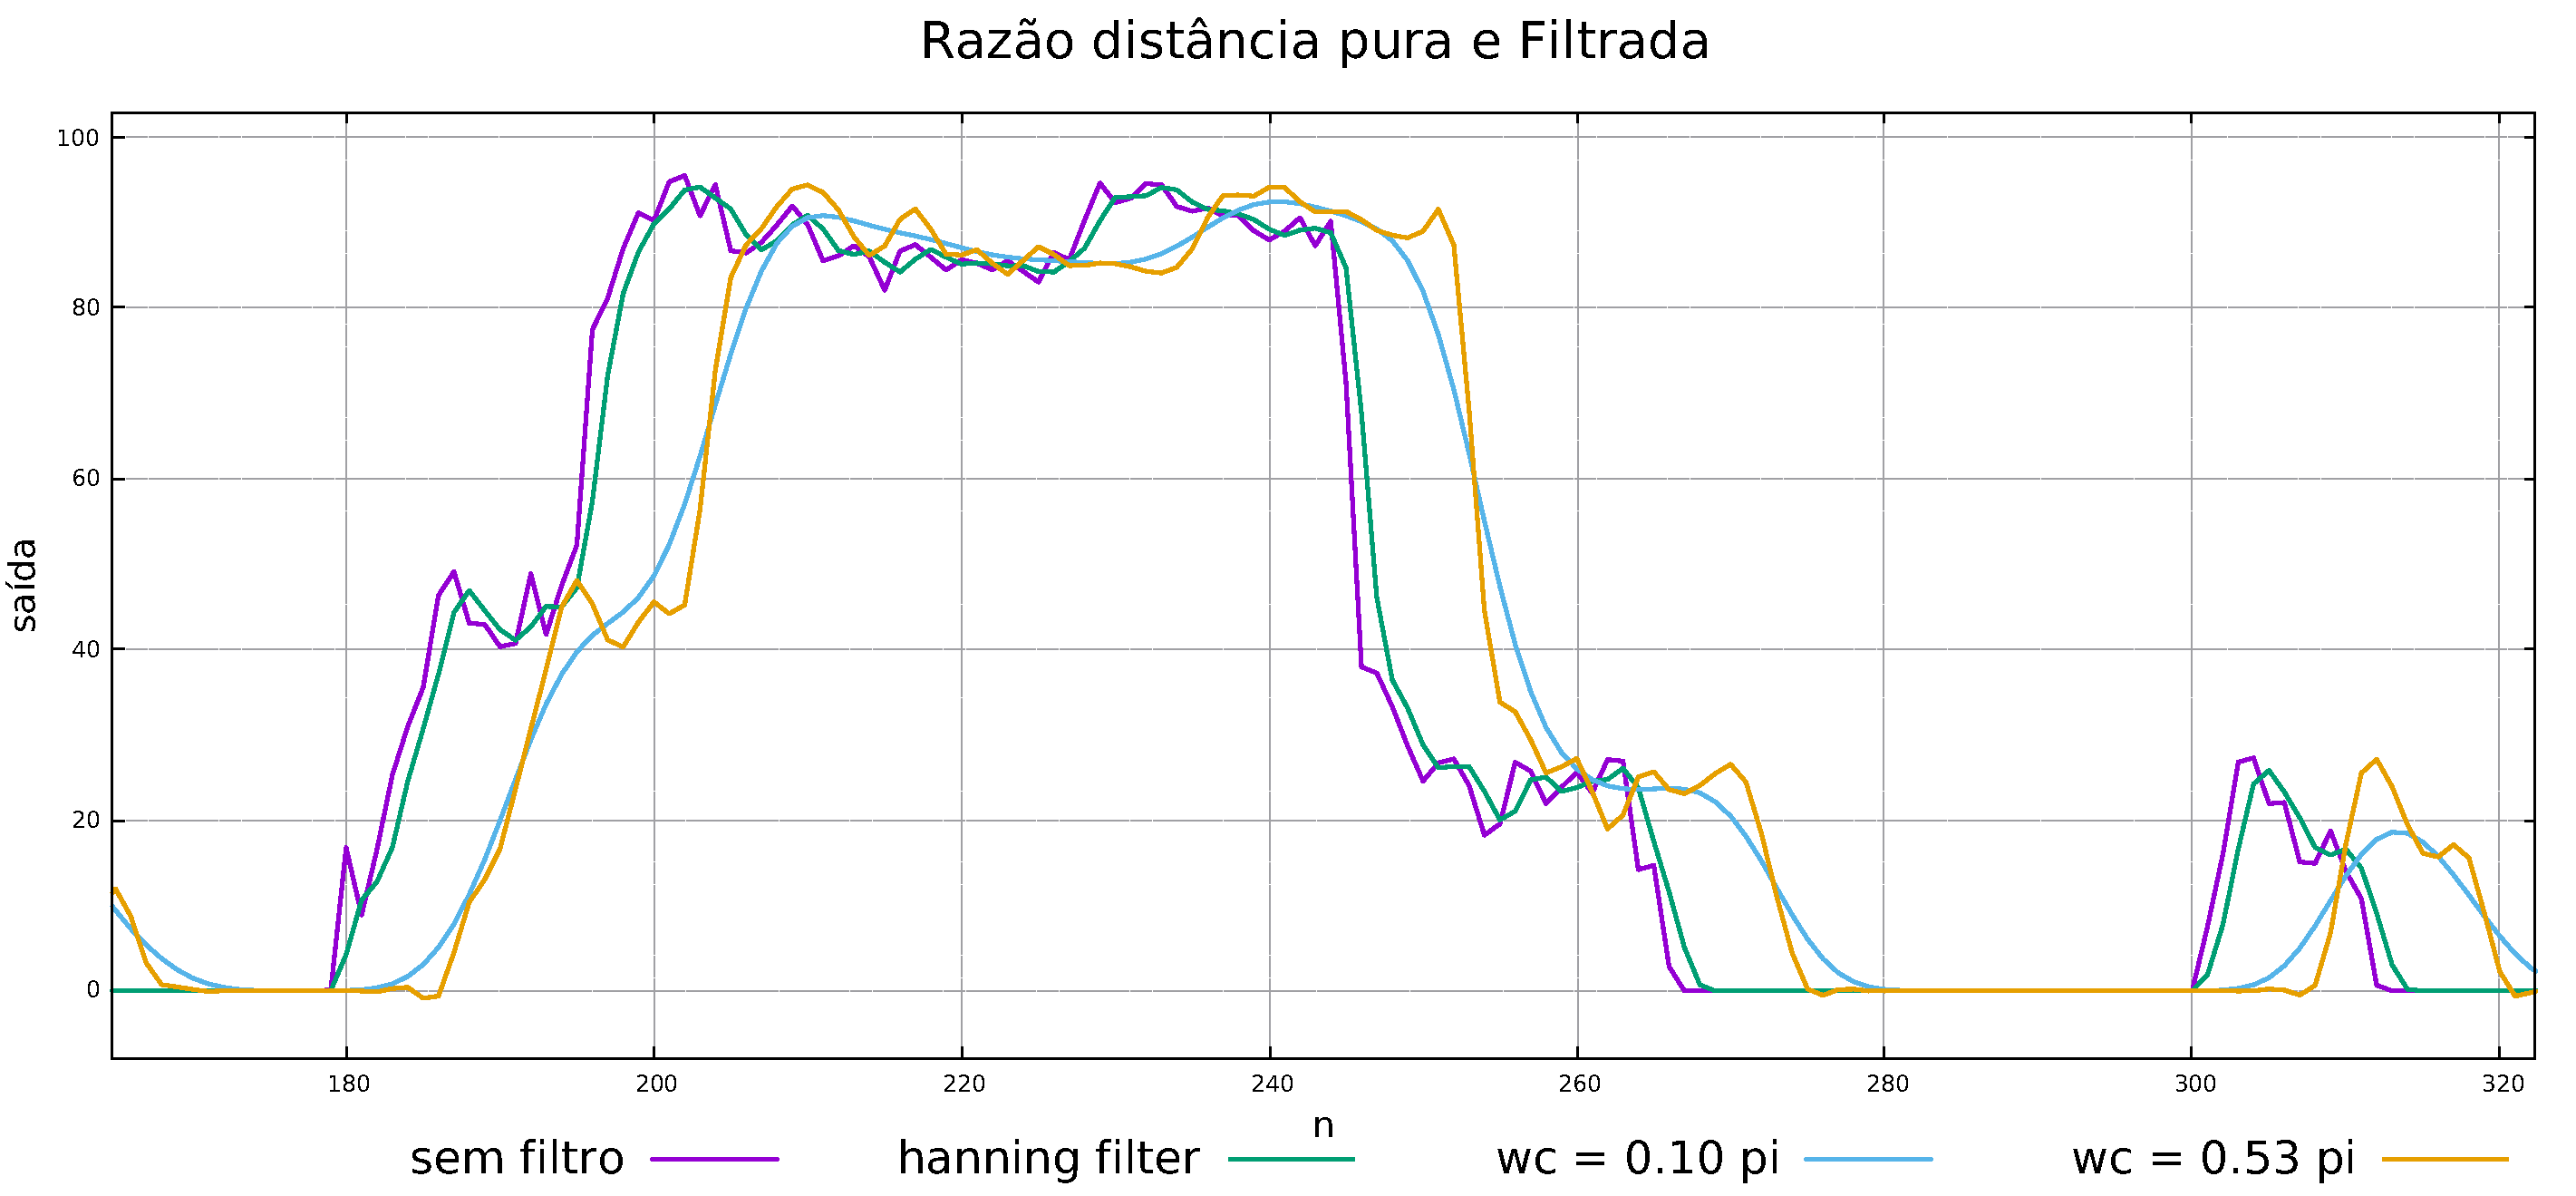
\includegraphics[width = 0.8\textwidth, keepaspectratio]{./img/filter-result-smile.pdf}
        \caption{Resultado da resposta ao sinal dos filtros projetados para o movimento do sorriso}
      \end{figure}
              
  \end{itemize} 
\end{frame}


\begin{frame}
\frametitle{Mistura de Poses}

	\begin{figure}
        \centering
        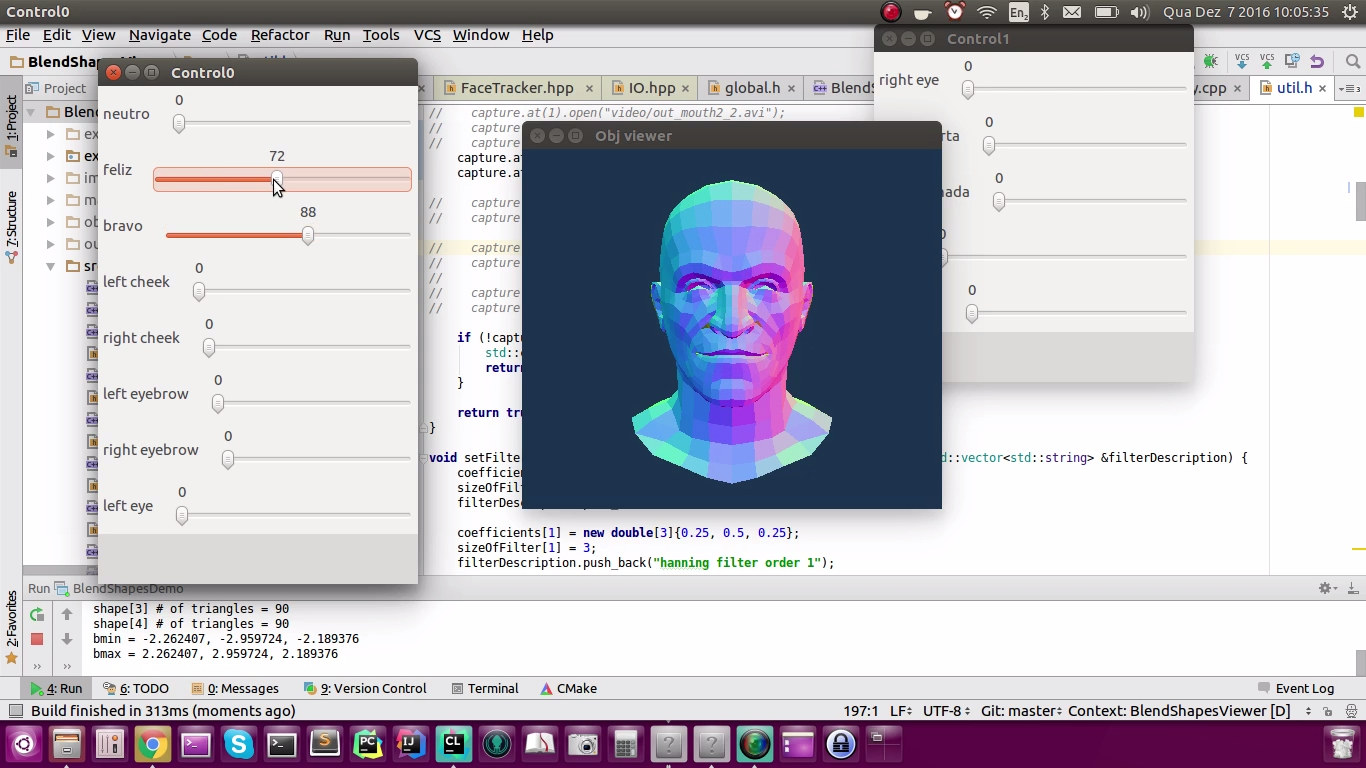
\includegraphics[width = 0.8\textwidth, keepaspectratio]{./img/blend-demo.png}
      \end{figure}
 
\end{frame}

\begin{frame}
\frametitle{Resultado Final} 

	\begin{figure}
        \centering
        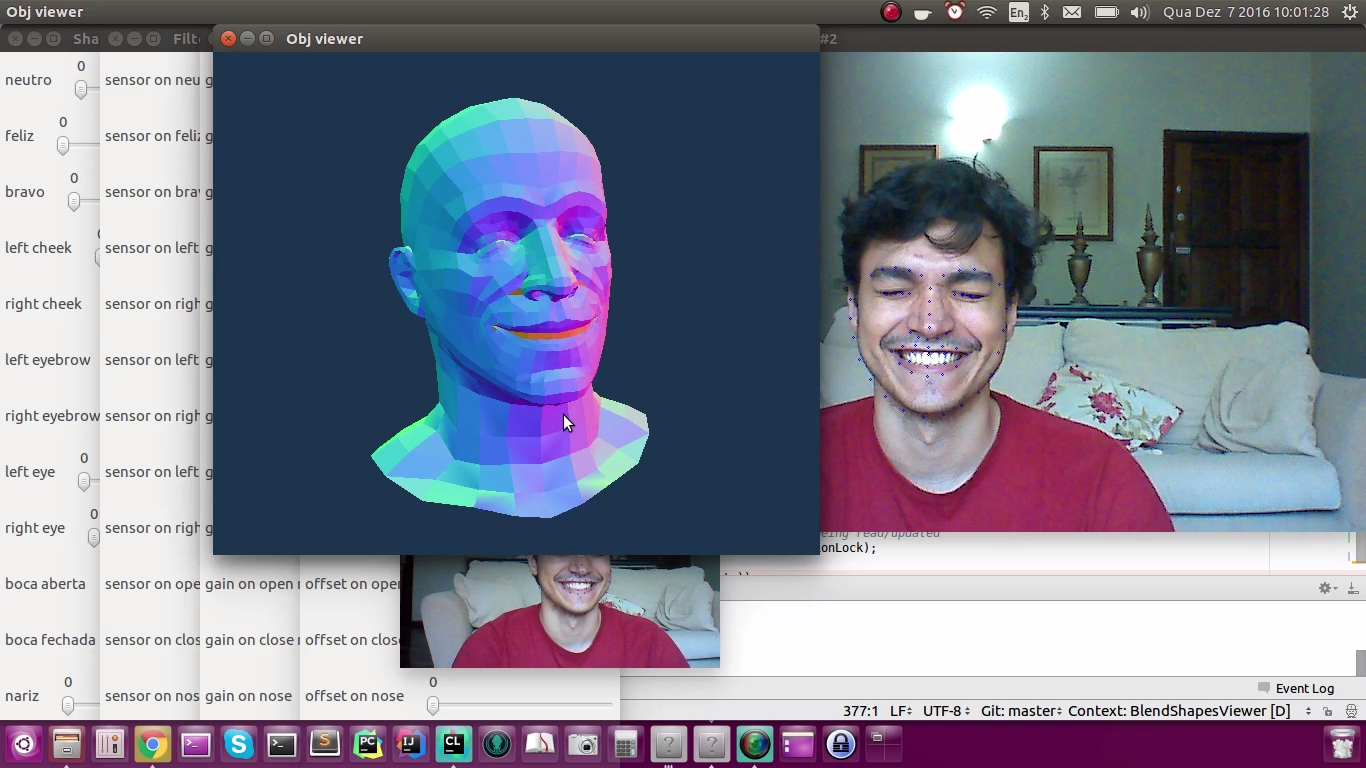
\includegraphics[width = 0.8\textwidth, keepaspectratio]{./img/result-0.png}
      \end{figure}

\end{frame}


\begin{frame}
\frametitle{Resultado Final}

	\begin{figure}
        \centering
        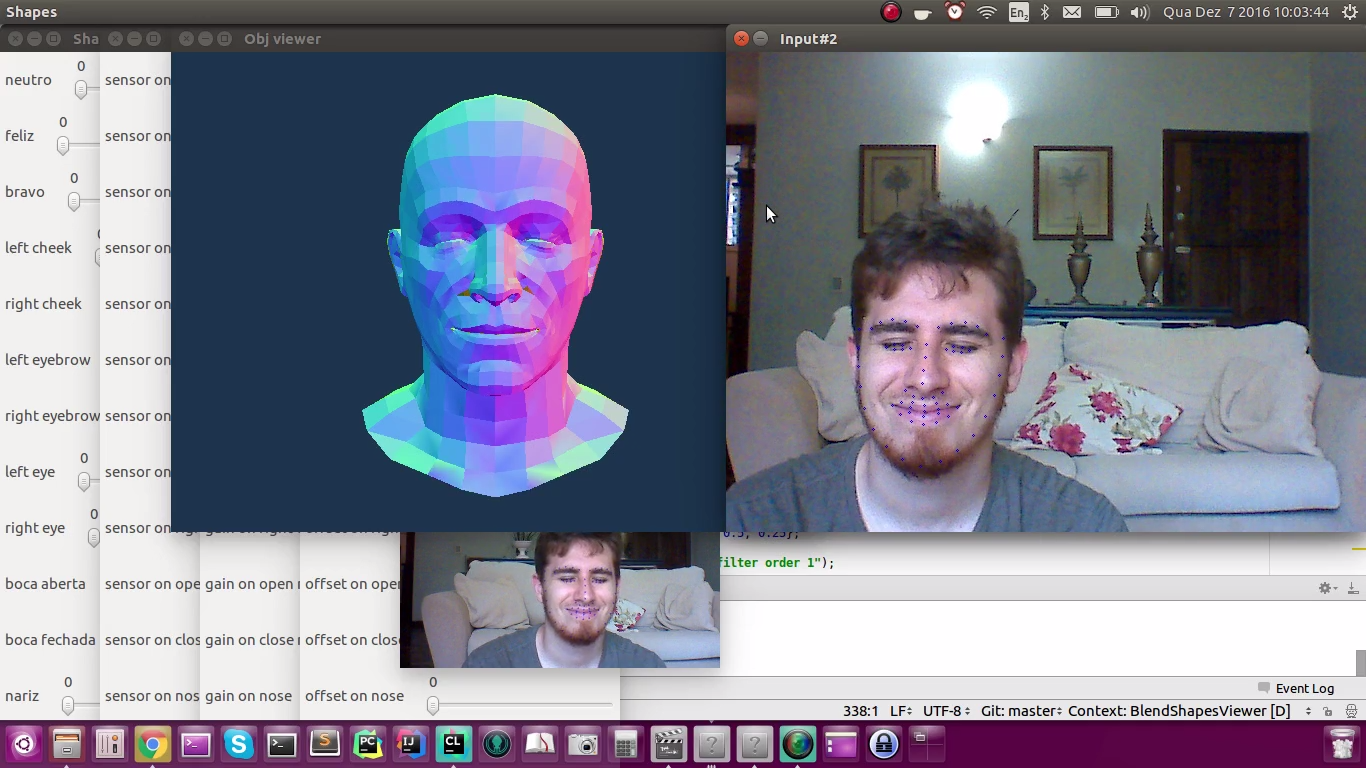
\includegraphics[width = 0.8\textwidth, keepaspectratio]{./img/result-1.png}
      \end{figure}
\end{frame}


\begin{frame}
\frametitle{Conclusões}
  \begin{itemize}
      \item Análise:
      Foi possível desenvolver uma ferramenta para animação computacional de \textbf{baixo custo}.
      \begin{itemize}
         \item Equipamento barato.
     	 \item Não é necessário ambiente controlado (ex: iluminação, background).
     	 \item Sem marcadores.
     	 \item Funcionamento independe do formato da face do ator (ex: gênero, idade, cor de pele).              
  	  \end{itemize} 
      
      \item Trabalhos Futuros:
      \begin{itemize}
         \item Modelos mais detalhados.
     	 \item Outros métodos para detecção de movimento em certas áreas da face.
     	 \item Uso de detectores de nuvens de pontos (ex: Kinect).           
  	  \end{itemize} 
              
  \end{itemize} 
\end{frame}


\begin{frame}

  Perguntas?
              
\end{frame}


\end{document}
